
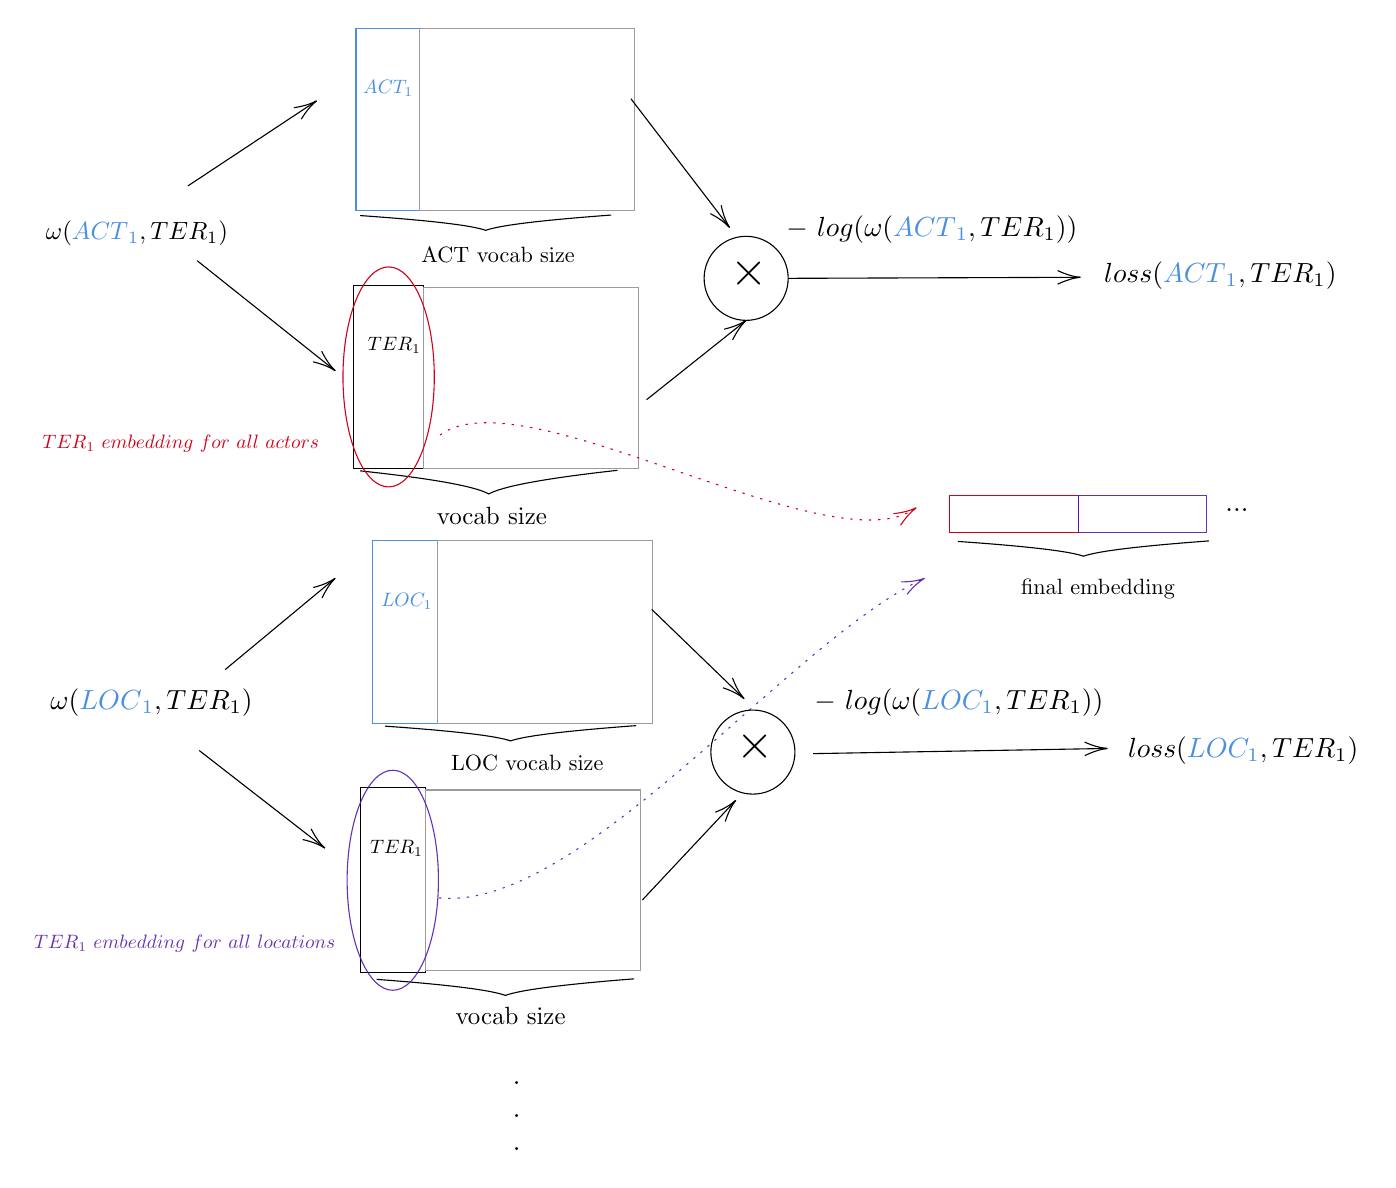
\begin{tikzpicture}[x=0.75pt,y=0.75pt,yscale=-1,xscale=1]
%uncomment if require: \path (0,573); %set diagram left start at 0, and has height of 573

\draw    (373.75,127.5) -- (514.5,127) ;
\draw [shift={(514.5,127)}, rotate = 539.8] [color={rgb, 255:red, 0; green, 0; blue, 0 }  ]   (0,0) .. controls (3.31,-0.3) and (6.95,-1.4) .. (10.93,-3.29)(0,0) .. controls (3.31,0.3) and (6.95,1.4) .. (10.93,3.29)   ;

\draw    (84.5,83) -- (146.5,42) ;
\draw [shift={(146.5,42)}, rotate = 506.52] [color={rgb, 255:red, 0; green, 0; blue, 0 }  ]   (0,0) .. controls (3.31,-0.3) and (6.95,-1.4) .. (10.93,-3.29)(0,0) .. controls (3.31,0.3) and (6.95,1.4) .. (10.93,3.29)   ;

\draw  [color={rgb, 255:red, 74; green, 144; blue, 226 }  ,draw opacity=1 ]  (165.5, 7) rectangle (196, 95)   ;
\draw    (164.5, 131) rectangle (198, 219)   ;
\draw  [color={rgb, 255:red, 155; green, 155; blue, 155 }  ,draw opacity=1 ]  (196, 7) rectangle (299.5, 95)   ;
\draw  [color={rgb, 255:red, 155; green, 155; blue, 155 }  ,draw opacity=1 ]  (198, 132) rectangle (301.5, 219)   ;
\draw [rotate around= { 89.88: (229.51, 225.75)
    }]  (223.89,163.75) .. controls (227.64,198.19) and (231.38,218.86) .. (235.13,225.75) .. controls (231.38,232.64) and (227.64,253.31) .. (223.89,287.75) ;
\draw [rotate around= { 89.88: (228.01, 100.75)
    }]  (224.39,40.25) .. controls (226.8,73.86) and (229.22,94.03) .. (231.63,100.75) .. controls (229.22,107.47) and (226.8,127.64) .. (224.39,161.25) ;
\draw    (353.5, 127.5) circle [x radius= 20.25, y radius= 20.25]  ;
\draw    (305.5,186) -- (353.5,147.75) ;
\draw [shift={(353.5,147.75)}, rotate = 501.45] [color={rgb, 255:red, 0; green, 0; blue, 0 }  ]   (0,0) .. controls (3.31,-0.3) and (6.95,-1.4) .. (10.93,-3.29)(0,0) .. controls (3.31,0.3) and (6.95,1.4) .. (10.93,3.29)   ;

\draw    (298,41) -- (345.5,103) ;
\draw [shift={(345.5,103)}, rotate = 232.54] [color={rgb, 255:red, 0; green, 0; blue, 0 }  ]   (0,0) .. controls (3.31,-0.3) and (6.95,-1.4) .. (10.93,-3.29)(0,0) .. controls (3.31,0.3) and (6.95,1.4) .. (10.93,3.29)   ;

\draw    (90,355) -- (150.5,402) ;
\draw [shift={(150.5,402)}, rotate = 217.84] [color={rgb, 255:red, 0; green, 0; blue, 0 }  ]   (0,0) .. controls (3.31,-0.3) and (6.95,-1.4) .. (10.93,-3.29)(0,0) .. controls (3.31,0.3) and (6.95,1.4) .. (10.93,3.29)   ;

\draw    (102.5,316) -- (155.5,272) ;
\draw [shift={(155.5,272)}, rotate = 500.3] [color={rgb, 255:red, 0; green, 0; blue, 0 }  ]   (0,0) .. controls (3.31,-0.3) and (6.95,-1.4) .. (10.93,-3.29)(0,0) .. controls (3.31,0.3) and (6.95,1.4) .. (10.93,3.29)   ;

\draw  [color={rgb, 255:red, 74; green, 144; blue, 226 }  ,draw opacity=1 ]  (173.5, 254) rectangle (205, 342)   ;
\draw    (167.5, 373) rectangle (199, 462)   ;
\draw  [color={rgb, 255:red, 155; green, 155; blue, 155 }  ,draw opacity=1 ]  (205, 254) rectangle (308.5, 342)   ;
\draw  [color={rgb, 255:red, 155; green, 155; blue, 155 }  ,draw opacity=1 ]  (199, 374) rectangle (302.5, 461)   ;
\draw [rotate around= { 89.88: (237.51, 469.07)
    }]  (233.57,407.07) .. controls (236.2,441.51) and (238.82,462.18) .. (241.44,469.07) .. controls (238.82,475.95) and (236.2,496.62) .. (233.57,531.07) ;
\draw    (356.75, 355.75) circle [x radius= 20.25, y radius= 20.25]  ;
\draw    (303.5,427) -- (348.5,379) ;
\draw [shift={(348.5,379)}, rotate = 493.15] [color={rgb, 255:red, 0; green, 0; blue, 0 }  ]   (0,0) .. controls (3.31,-0.3) and (6.95,-1.4) .. (10.93,-3.29)(0,0) .. controls (3.31,0.3) and (6.95,1.4) .. (10.93,3.29)   ;

\draw    (308,287) -- (352.5,330) ;
\draw [shift={(352.5,330)}, rotate = 224.02] [color={rgb, 255:red, 0; green, 0; blue, 0 }  ]   (0,0) .. controls (3.31,-0.3) and (6.95,-1.4) .. (10.93,-3.29)(0,0) .. controls (3.31,0.3) and (6.95,1.4) .. (10.93,3.29)   ;

\draw [rotate around= { 89.88: (240.01, 346.75)
    }]  (236.39,286.25) .. controls (238.8,319.86) and (241.22,340.03) .. (243.63,346.75) .. controls (241.22,353.47) and (238.8,373.64) .. (236.39,407.25) ;
\draw  [color={rgb, 255:red, 208; green, 2; blue, 27 }  ,draw opacity=1 ]  (181.25, 175) circle [x radius= 22, y radius= 53]  ;
\draw  [color={rgb, 255:red, 82; green, 21; blue, 168 }  ,draw opacity=0.88 ]  (183.25, 417.5) circle [x radius= 22, y radius= 53]  ;
\draw [color={rgb, 255:red, 208; green, 2; blue, 27 }  ,draw opacity=1 ] [dash pattern={on 0.84pt off 2.51pt}]  (206,203) .. controls (246,173) and (395.5,268) .. (435.5,238) ;
\draw [shift={(435.5,238)}, rotate = 508.65] [color={rgb, 255:red, 208; green, 2; blue, 27 }  ,draw opacity=1 ]   (0,0) .. controls (3.31,-0.3) and (6.95,-1.4) .. (10.93,-3.29)(0,0) .. controls (3.31,0.3) and (6.95,1.4) .. (10.93,3.29)   ;

\draw [color={rgb, 255:red, 82; green, 21; blue, 168 }  ,draw opacity=0.88 ] [dash pattern={on 0.84pt off 2.51pt}]  (205.5,426) .. controls (273.5,433) and (375.5,301) .. (439.5,272) ;
\draw [shift={(439.5,272)}, rotate = 514.4] [color={rgb, 255:red, 82; green, 21; blue, 168 }  ,draw opacity=0.88 ]   (0,0) .. controls (3.31,-0.3) and (6.95,-1.4) .. (10.93,-3.29)(0,0) .. controls (3.31,0.3) and (6.95,1.4) .. (10.93,3.29)   ;

\draw  [color={rgb, 255:red, 208; green, 2; blue, 27 }  ,draw opacity=1 ]  (451.5, 232) rectangle (513.5, 250)   ;
\draw  [color={rgb, 255:red, 82; green, 21; blue, 168 }  ,draw opacity=0.88 ]  (513.5, 232) rectangle (575.5, 250)   ;
\draw    (89,119) -- (155.5,172) ;
\draw [shift={(155.5,172)}, rotate = 218.55] [color={rgb, 255:red, 0; green, 0; blue, 0 }  ]   (0,0) .. controls (3.31,-0.3) and (6.95,-1.4) .. (10.93,-3.29)(0,0) .. controls (3.31,0.3) and (6.95,1.4) .. (10.93,3.29)   ;

\draw    (385.75,356.5) -- (527.5,354) ;
\draw [shift={(527.5,354)}, rotate = 538.99] [color={rgb, 255:red, 0; green, 0; blue, 0 }  ]   (0,0) .. controls (3.31,-0.3) and (6.95,-1.4) .. (10.93,-3.29)(0,0) .. controls (3.31,0.3) and (6.95,1.4) .. (10.93,3.29)   ;

\draw [rotate around= { 89.88: (516.01, 257.75)
    }]  (512.39,197.25) .. controls (514.8,230.86) and (517.22,251.03) .. (519.63,257.75) .. controls (517.22,264.47) and (514.8,284.64) .. (512.39,318.25) ;

\draw (60,106) node [scale=0.9] [align=left] {$\omega (\textcolor[rgb]{0.29,0.56,0.89}{ACT}\textcolor[rgb]{0.29,0.56,0.89}{_{1}} ,TER_{1})$};
\draw (181,36) node [scale=0.7,color={rgb, 255:red, 74; green, 144; blue, 226 }  ,opacity=1 ]  {$ACT_{1}$};
\draw (582,126) node  [align=left] {$loss(\textcolor[rgb]{0.29,0.56,0.89}{ACT}\textcolor[rgb]{0.29,0.56,0.89}{_{1}} ,TER_{1})$};
\draw (184,160) node [scale=0.7]  {$TER_{1}$};
\draw (234,116) node [scale=0.8] [align=left] {ACT vocab size};
\draw (231,242) node [scale=0.9] [align=left] {vocab size};
\draw (67,332) node  [align=left] {$\omega (\textcolor[rgb]{0.29,0.56,0.89}{LOC}\textcolor[rgb]{0.29,0.56,0.89}{_{1}} ,TER_{1})$};
\draw (190,283) node [scale=0.7,color={rgb, 255:red, 74; green, 144; blue, 226 }  ,opacity=1 ]  {$LOC_{1}$};
\draw (185,402) node [scale=0.7]  {$TER_{1}$};
\draw (248,361) node [scale=0.8] [align=left] {LOC vocab size};
\draw (240,483) node [scale=0.9] [align=left] {vocab size};
\draw (243,531) node  [align=left] {.\\.\\.};
\draw (81,207) node [scale=0.7,color={rgb, 255:red, 208; green, 2; blue, 27 }  ,opacity=1 ]  {$TER_{1} \ embedding\ for\ all\ actors$};
\draw (83,448) node [scale=0.7,color={rgb, 255:red, 82; green, 21; blue, 168 }  ,opacity=0.88 ]  {$TER_{1} \ embedding\ for\ all\ locations$};
\draw (590,239) node  [align=left] {...};
\draw (443,104) node  [align=left] {$-\ log( \omega (\textcolor[rgb]{0.29,0.56,0.89}{ACT}\textcolor[rgb]{0.29,0.56,0.89}{_{1}} ,TER_{1}))$};
\draw (593,355) node  [align=left] {$loss(\textcolor[rgb]{0.29,0.56,0.89}{LOC_{1}} ,TER_{1})$};
\draw (456,332) node  [align=left] {$-\ log( \omega (\textcolor[rgb]{0.29,0.56,0.89}{LOC_{1}} ,TER_{1}))$};
\draw (523,277) node [scale=0.8] [align=left] {final embedding};
\draw (355,125) node [scale=1.7280000000000002]  {$\times $};
\draw (358,353) node [scale=1.7280000000000002]  {$\times $};

\end{tikzpicture}


